\chapter{System Methodology}
% \section{IoT System}
% Here, we are using a bread board (see figure \ref{fig:node}) for connecting the node mcu with the sensors.  We have a dht11 sensor whose positive and negative portion are connected to the positive and negative portion of node mcu respectively. The data section of the sensor is connected to the D5 pin of the node mcu. The SDA and SCL of the monitor are connected to the D2 and D1 pins of the node mcu respectively. The other sensor’s (Optimal Pulse sensor, Glucometer, GSR, ECG Sensor, MPU 6050 Accelarometer Gyroscope, Sphygmomanometer, Pulse Oxymetry) positive and negative portion are also connected to the positive and negative portion of node mcu respectively.

% \begin{itemize}
% \item	DHT11 temperature humidity sensor, Optimal Pulse sensor, Glucometer, GSR, ECG Sensor, MPU 6050 Accelarometer Gyroscope, Sphygmomanometer and Pulse Oxymetry to sense the data from human body and send it to microcontroller 
% \item 	We use node mcu ESP 8266 for sending the collected data in the cloud database “ThingSpeak” 
% \item  Data will be sent to the application via wireless network from the cloud server. 
% \item  Specified doctor and caretaker can be able to monitor the collected data of the patient's also in the mobile application platform.
% \end{itemize}
% \begin{figure}[ht]
%     \centering
%      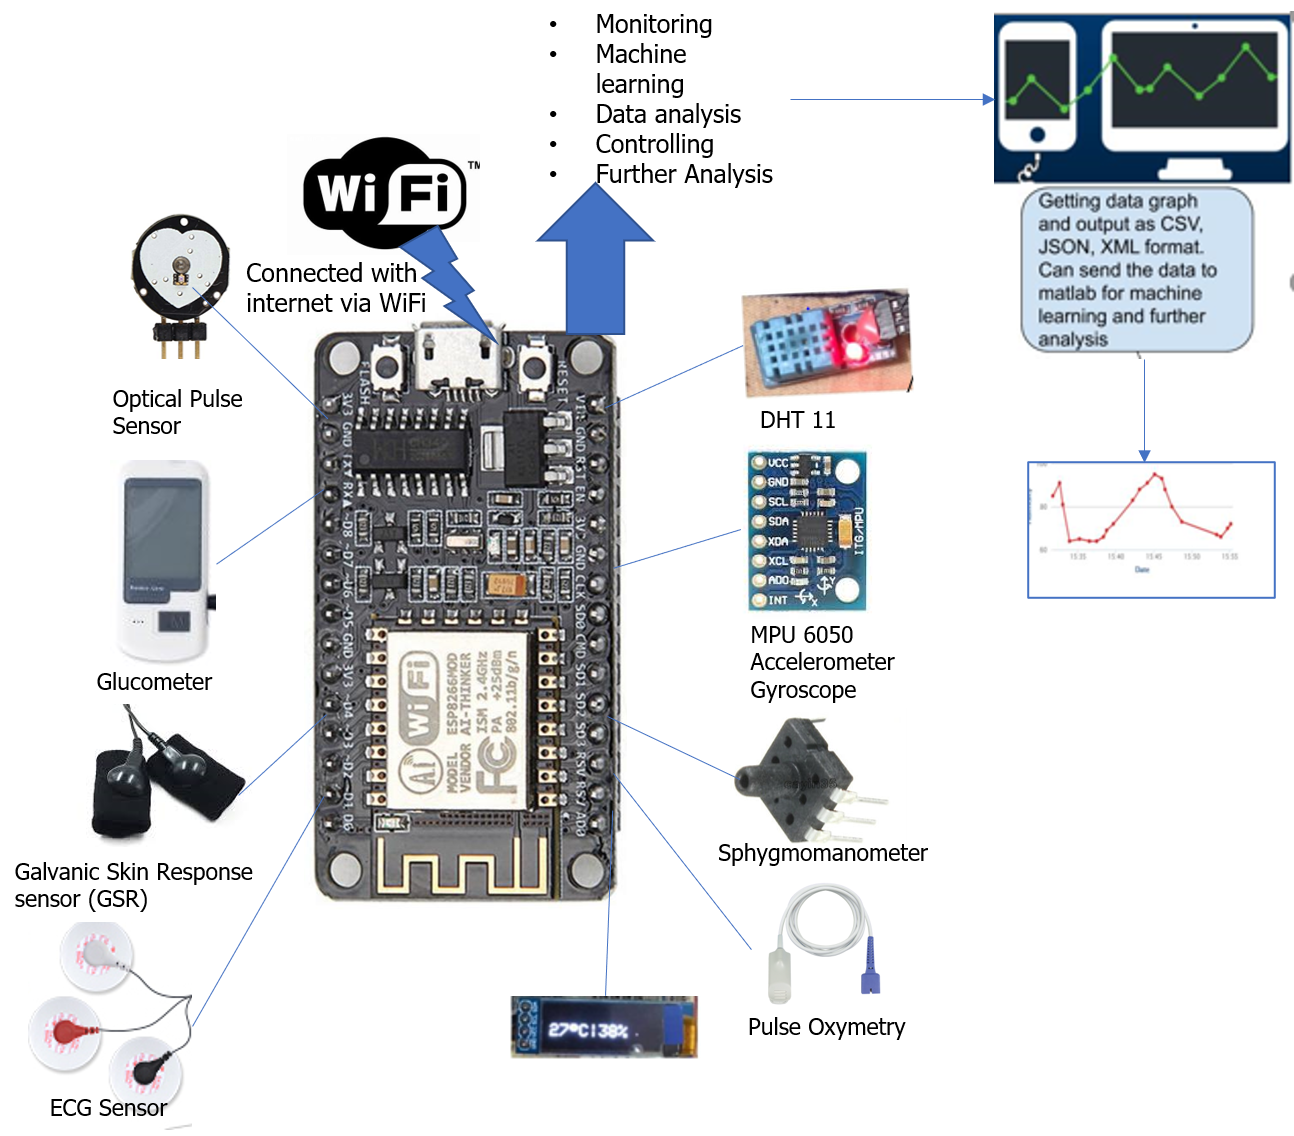
\includegraphics[width=4.25in]{Chap4/Circuit Diagram.png}
%      \caption{Conceptual Framework of IoT system components}
%      \label{fig:node}
% \end{figu
% \section{Fall Detection}
In this chapter, we represent our Machine Learning architecture which intrigrates data collection, data preprocessing, feature extraction and ML algorithm to detect a fall event. Two dataset named UR fall detection dataset and Open labeled dataset are used in our framework. To extract features from these dataset we have used data pre processing techniques. From them we splitted training set and test set of data where train data have been classified by Machine Learning classifiers.

\vspace{0.5cm}
Figure \ref{fig:Fall_model} shows Fall detection architecture and datasets used to train the model using these Ur fall detection and open labelled dataset. Firstly, We have applied batch normalization in both datasets 
to boost the pace at which network learns and re-scaling and re-centering the input layer would make for a higher learning rate. The RNN layer can then be added to all datasets.Then we have applied the layer on both datasets that transforms the RNN outputs to our desired form is completely connected. Just before the output layer, Softmax is added, which allocate decimal probabilities to add up to 1. The final fusion of information from both datasets are used to detect the fall accurately.


% to improve
% the speed at which the network trains, and it will allows higher learning rate by re-scaling and re-centering the input layer. Then RNN layer is applied on both datasets.



% Fully Connected layer on both dataset which converts the RNN outputs to our desired shape. Softmax is implemented just before the output layer which
% assign decimal probabilities that must sum to 1. At last knowledge fusion from both datasets 
% are used to detect the fall appropriately.

\vspace{0.5cm}
\textbf{Batch Normalization: }Batch normalization is a method for preparing extremely deep neural networks which normalize the contributions to a layer for every small bunch. It also has the impact of stabilizing the method of learning and significantly decreasing the amount of cycles of learning needed to prepare deep networks. Normalizing the contributions to the layer affects the preparation of the model decreasing the quantity of ages needed. It may even have a parallelizing impact, similar to such activation regularization, decreasing error rate. In our data sets there are too many data inputs. And we don’t need all the data together. So we normalize this sets in a mini batch and then use it further implementation.

\vspace{0.5cm}
\textbf{RNN Layer: } Data has to be passed through the layers of RNN to modelling sequence the data. The three layers of RNN is defined the dataset. RNN, which solved this problem with the aid of a Secret Layer, came into its' presence.

\vspace{0.5cm}
\textbf{SoftMax: }The softmax transforms a vector of genuine qualities into a vector of genuine qualities that total to 1. The info esteems can be positive, negative, zero, or more prominent than one, yet the softmax changes them into values somewhere in the range of 0 and 1, so they can be deciphered as probabilities.


\vspace{.5cm}
\textbf{Knowledge Fusion: }Knowledge fusion is a significant tool to find as well as cleanning the mistakes and errors which impending in the source of information and the numerous missteps during the time spent information extraction from sources.




% \section{Dataset Description}
% Two datasets named 
% UR dataset and Open 
% labeled dataset have been
% used in our system 
% (see Table \ref{resulttab:1}).
% UR fall detection dataset are developed by kepski 
% \emph{et al.}
% \cite{kwolek_human_2014}
% used seventy sequences
% where thirty are falls 
% and fourty are activities 
% of daily living (ADL).
% Two camera are used.
% One is front facing 
% and other is from 
% ceiling which provides 
% the top views of the scene. Kinect cameras and corresponding accelerometric data are used to record fall and one device(camera 0) are used to record ADL. IMU and PS Move devices are used to collect sensor data. Two types of falls, one from standing and other while sitting on a chair are described here. Besides picking object from ground, lying on the sofa and floor, normal walking, sitting down are the ADL. Data needed to extract features of UR are\\
% \begin{itemize}
%     \item \textbf{Height/Width}- Bounding box height to width ratio
%     \item \textbf{l/w} - Major to minor axis ratio
%     \item \textbf{H/Hmax} - A proportion expressing the height of the person's surrounding box in the current frame to the physical height of the person, projected onto the depth map  and
%     \item \textbf{Area} - A ratio expressing the person’s area in the image to the area at assumed distance to the camera.
% \end{itemize} 

% Wertner \emph{et al.} \cite{wertner_open_2015} has created a labelled dataset which can be used for mobile phone with the data of accelerometer and gyroscope sensor. An orientation software based sensor is used to derive data from the accelerometer and geomagnetic field sensor which is attached to the mobile phone and the data is recorded by the mobile phone. Data needed to extract features of Open labelled are:

% \begin{itemize}
%     \item \textbf{Acceleration of devices:} Acceleration is stored as 3D vector indicating acceleration along each device axis, not including gravity. It can be calculated as
%     \begin{equation}
%         a_{xyz}=\sqrt{x^2+y^2+z^2}
%     \end{equation}
    
%      \item \textbf{Orientation of devices:} Orientation is stored as 3D vector of angles azimuth, pitch and roll.
% \end{itemize}


% \begin{figure}[!ht]
%     \centering
%     \includegraphics[scale=1.0]{Chap5/Fig03 B245.pdf}
%     \caption{Proposed Fall Detection Architecture and datasets used to train the model. (A) shows features used in the proposed RNN model and (B) illustrate the RNN architecture}
%     \label{fig:Fall_model}
% \end{figure}


% \begin{table}[!ht]
%     \centering
%     \scriptsize
%     \begin{tabular}{lp{1in}p{1.5in}cc}\toprule
%         Dataset & Sensor used &No of record & Training & Testing\\ \midrule
%          Open Labelled
% & Smart phone  &159300 records of acceleration
% and 159300 records of orientation&223020 &95580\\ \midrule
%         UR & Camera &70 (30 falls and 40 activities of daily living) sequences& 49&21\\ \bottomrule
%     \end{tabular}
%     \caption{Information about the dataset used in this study.}
%     \label{resulttab:1}
% \end{table}

 \section{Dataset Description}
UR fall detection dataset and Open Labelled dataset are used in our system.
(see Table \ref{resulttab:1}).
 kepski 
\emph{et al.} developed the UR fall detection dataset.
\cite{kwolek_human_2014}. There are total seventy video sequences in the dataset where thirty video sequences indicate fall activities and  fourty video sequences are activities 
of Daily Living (ADL).
To make this dataset two cameras are used in a home environment. Among them One is front facing camera and the other is from ceiling of the house which provides the top views of the scene.  Kinect cameras developed by microsoft and corresponding accelerometric data collected from the sensors are used to capture and record fall. Kinect camera are consist of three vital parts and they are depth sensor, VGA camera that used RGB color and a multi array microphone. The camera sensor recognizes the color components of red, green,
and blue. It also recognise facial features and motion. Another One device(camera 0) are used to record ADL. Sensor data are collected by the IMU and PS move devices. This dataset describes two type of falls. They are Fall from the standing and fall while sitting on a chair. Activities of Daily Life(ADL) are recognised as picking an item from ground, lying down on a floor and sofa, normal walking on the floor and sitting down from standing.So the Data needed to extract features from UR fall detection dataset are given below:\\
\begin{itemize}
    \item \textbf{Height/Width}- Bounding box height to width ratio. While falling, a person's height to width ratio changes very fast. If the system can detect the ratio and then compare it with the given threshold value then the system can easily detect if a fall has occurred or not. 
    
    \item \textbf{L/W} - This features represent the Major to minor axis ratio of the bounded box.
    
    \item \textbf{H/Hmax} - This features express the ratio of person height in the bounded box of the current image frame to the actual physical height of the person, which have been plotted onto the depth map. 
    
    \item \textbf{Area} - The ratio of the person's area in the image frame
to the area at the distance assumed by the camera. Sudden change in the ratio of area can identify fall events.
\end{itemize} 

\vspace{0.5cm}
 A labelled dataset was developed by Wertner \emph{et al.} \cite{wertner_open_2015} where accelerometer and gyroscope sensor of a mobile phone are used to collect the data. To label the fall they selected falls in different directions at different speed. Fall activities like Fast forward fall is labelled as 'Stumbling', Fast backward fall is labelled as 'Slipping', and Slow lateral fall is labelled as 'Sliding' and 'Getting Unconscious'. Non fall activities are labelled as 'walking', 'standing', 'stopping', 'sit down', 'sit down quickly', 'Get up', 'Stairs up', 'Stairs down', 'Bend forward', 'Bend backward', 'Lying on the floor'. They are called as Activity of Daily Life(ADL). To collect the data an orientation software based sensor and a geomagnetic field sensor which is attached in a cell phone are used.  Then data is also recorded by the mobile phone. Data needed to extract features of Open labelled are:

\begin{itemize}
    \item \textbf{Acceleration of devices:} 
    
An accelerometer is an electromechanical instrument often used calculate the powers of acceleration. Such factors can be rigid, like the constant gravitational force, or dynamic to detect acceleration or movements, as seems to be the case for certain portable devices. 

\vspace{0.5cm}
Acceleration is the calculation of the time-divided shift in velocity, or distance.
To evaluate the angle at which a system is inclined with respect to the Ground, a dynamic accelerometer tests the angular momentum. Users analyze how the system is going by sensing the sum of acceleration. Figure \ref{fig:Accel} Shows the Coordinate system of a accelerometer. 

\begin{figure}[!ht]
    \centering
    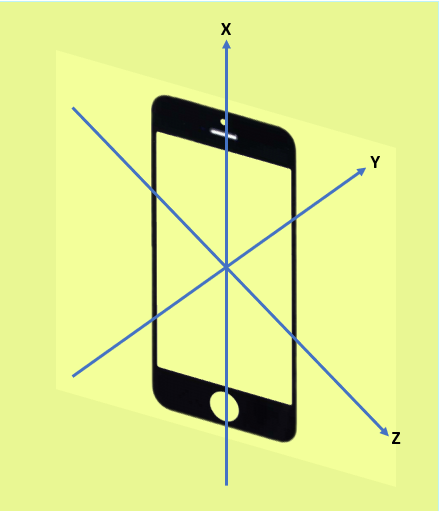
\includegraphics[scale=0.5]{Chap4/Capture.PNG}
    \caption{Coordinate System of an accelerometer}
    \label{fig:Accel}
\end{figure}

\vspace{0.5cm}
Conventional accelerometers consist of three dimensions, two with the choice of a third for 3D positioning to assess most two-dimensional motions. Usually, most smartphones make use of three-axis versions. The accuracy of these instruments is very high, since even very minute acceleration variations are meant to be calculated. The more robust the accelerometer is, the more effectively acceleration can be measured.

\vspace{0.5cm}
Acceleration is stored as 3D vector indicating acceleration along each device axis, not including gravity. It can be calculated as
    \begin{equation}
        a_{xyz}=\sqrt{x^2+y^2+z^2}
    \end{equation}
    
     \item \textbf{Orientation of devices:} 
     In terms of momentum, device orientation enables a device to sense its actual inclination. Orientation is determined using three angles that define the current orientation of the device: alpha, beta, and gamma. Figure \ref{fig:Gyro} shows the coordinate system of a gyroscope.
     
     \begin{figure}[!ht]
     \centering
     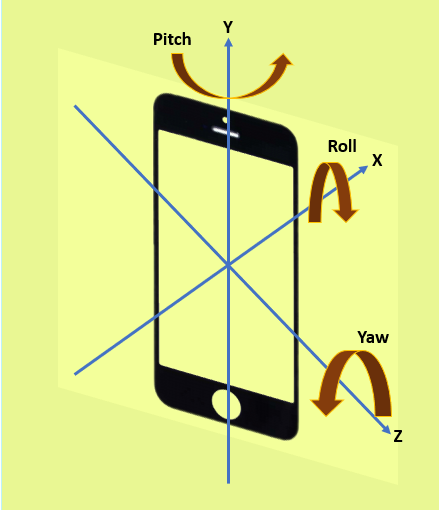
\includegraphics[scale=0.5]{Chap4/Orientation.PNG}
     \caption{Coordinate System of a gyroscope}
     \label{fig:Gyro}
     \end{figure}
     
 \vspace{0.5cm}    
The gyroscope can be used to estimate the tilt of pitch and roll (in degrees): 

On the Y-axis, pitch is rotation, meaning an object is tilted up or down. 
On the X-axis, roll is rotation, meaning an object is tilted right or left.
Yaw is rotation in Z-axis.

     Orientation is stored as 3D vector of angles azimuth, pitch and roll.
\end{itemize}


\begin{figure}[!ht]
    \centering
    \includegraphics[scale=1.0]{Chap4/Fig03 B245.pdf}
    \caption{Proposed Fall Detection Architecture and datasets used for model training. (A) shows features used in the proposed RNN model and (B) illustrate the RNN architecture}
    \label{fig:Fall_model}
\end{figure}




\begin{table}[!ht]
    \centering
    \scriptsize
    \begin{tabular}{lp{1in}p{1.5in}cc}\toprule
        Dataset & Sensor used &No of record & Training & Testing\\ \midrule
         Open Labelled
& Smart phone  &159300 records of acceleration
and 159300 records of orientation&223020 &95580\\ \midrule
        UR & Camera &70 (30 falls and 40 activities of daily living) sequences& 49&21\\ \bottomrule
    \end{tabular}
    \caption{Information about the dataset used in this study.}
    \label{resulttab:1}
\end{table}




\section{Feature Extraction}
In the fall detection scheme, a feature extraction module plays an essential role. Our emphasis was on the generation and collection of functionality to increase the fall detection rate. We have extracted features from UR and free labelled datasets in this analysis.
% A feature extraction module performs a significant role in the fall detection system. To enhance the fall detection rate, our focus was on the generation and selection of features.In this research we have extracted for features from UR and open labeled dataset.

 
It represents the variety of change of the magnitude of acceleration in x, y and z axis.


 \paragraph{\textbf{Variance of CV Acceleration:}}
 Coefficient of Variation indicates the degree of heterogeneity in comparison to the population's average. Only observations evaluated on an interval scale, that is, scales that have a relevant zero and thus allow a roughly similar comparison of two measurements, should be approximated for the coefficient of variation (division of one measurement by the other).
 
 Standard deviation of acceleration data is calculated then divided by it’s mean ($\mu$) ti get the coefficient of variation (CV).
%begin{math}
\begin{equation}
    \sigma_{xyz}=\frac{\sqrt{\sigma_x^2+\sigma_y^2+\sigma_z^2 }}{\mu}
\end{equation}
    

%\paragraph{\textbf{Position:}}
%The position If we integrate acceleration data, we will get the velocity. if, we again integrate velocity, thus we will find the position.

%\begin{equation}
%    r=\int\sqrt{(\int a_x(t)dt)^2+(\int(a_y (t)dt)^2+(\int(a_z (t)dt)^2 )})dt
%\end{equation}
\paragraph{\textbf{Variation in motion vector:}}

In the motion estimation process, a motion vector is the main component. It is used in another frame, called the reference picture, to represent a macroblock in an image based on the location of this macroblock.

By discovering a correlation between frames at time t, and  frames at time t-1, where t is the frame index in a video signal and thus motion vector' is estimated.

While a person is falling his body is in a motion. So during a fall event the magnitude of the motion variation will be high. The motion variation will be increasing rapidly from it's normal value and the value will be 0 when fall take place.
To calculate the magnitude of motion variation equation is given below:

\begin{equation}
     m_{xyz}=\sqrt{(m_x^2 +m_y^2+m_z^2 )}
\end{equation}

\paragraph{\textbf{Polar Angle Ratio:}}
While a person is falling the polar angle will be changed also. The polar angle which is denoted by $\theta$  is the anticlockwise orientation in the region from the x-axis at which a position is located in the xy-plane.


\begin{figure}[!ht]
    \centering
    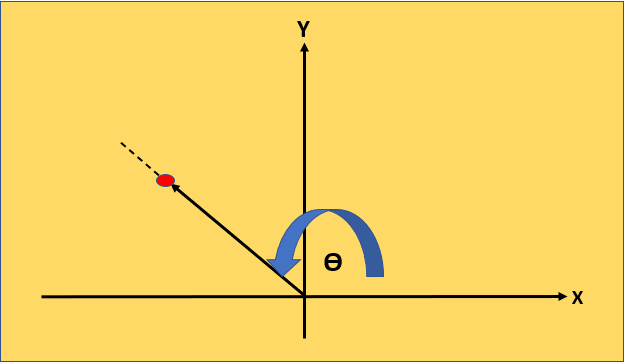
\includegraphics[scale=0.5]{Chap4/Polar.PNG}
    \caption{Polar Angle}
    \label{fig:Polar Angle}
\end{figure}

Polar angle ratio from accelerometer data can be calculated as follows:
\begin{equation}
    \cos^{-1}\left(\frac{z}{\sqrt{x^2+y^2+z^2}}\right)
\end{equation}


 
 This polar angle ratio will (see fig \ref{fig:Polar Angle}) reflects the  sudden transition of a human body angle which will suggest that a fall has taken place. Moreover, sudden change is reflected by the ratio of instant angle of the body and it's past values within a short amount of time.


 \paragraph{\textbf{Difference Between Polar Angle:}}
 $\Delta\theta$ represents the difference between polar angle which helps to detect large tilt angle variations. This can identify if a fall has occurred or not.

% \section{ML Algorithm}
% \paragraph{Recurrent Neural Network (RNN):} RNN mainly used for supervised time series analysis is a machine learning algorithm where outputs of the previous step are used for the inputs of next step. Hidden state are the most important feature of RNN. RNN with convolutionary layers are used to expand the successful neighborhood of pixels.

% \paragraph{Random Forrest (RF):} Random forrest is a supervised learning algorithm which is a combination of decision trees where the forrest is build by an assemble of decision trees to increase the overall result by combining learning models. Here the input is evaluated by the decision tree forest and the output class is measured as the tree's response class.

% \paragraph{Support Vector Machine (SVM):} SVM which is mostly used for classification is a machine learning algorithm which helps to solve pattern recognition. Coordinates of individual observations are represented by support vector. It is a frontier that separates both classes at its best. Each data item is ploted in an n-dimensional space where n indicates the number of features we have and the value of each feature represent the value of a particular coordinates.

\section{Model Training}
To train our model we have splitted both the datasets named 'UR Fall Detection Dataset' and 'Open Labelled Dataset' into two parts where 70\% data from each dataset is used for training purpose and the remaining 30\% is used for testing purpose. We have used 5-fold cross validation to resampling our data. For the 5-fold cross validation, we used random partition from the datasets.

% \section{Node mcu ESP 8266 part: } Here, we are using a bread board for connecting the node mcu with the sensors.  We have a dht11 sensor whose positive and negative portion are connected to the positive and negative portion of node mcu respectively. The data section of the sensor is connected to the D5 pin of the node mcu. The SDA and SCL of the monitor are connected to the D2 and D1 pins of the node mcu respectively. The other sensor’s (Optimal Pulse sensor, Glucometer, GSR, ECG Sensor, MPU 6050 Accelarometer Gyroscope, Sphygmomanometer, Pulse Oxymetry) positive and negative portion are also connected to the positive and negative portion of node mcu respectively.

% We have used:

% \begin{itemize}
%     \item	Dht11 temperature humidity sensor, Optimal Pulse sensor, Glucometer, GSR, ECG Sensor, MPU 6050 Accelarometer Gyroscope, Sphygmomanometer and Pulse Oxymetry to sense the data from human body and send it to microcontroller 
%      \item 	We use node mcu ESP 8266 for sending the collected data in the cloud database “Thingspeak” 
%       \item  We have send data to our cell phone via Wifi. 
%       \item It has been work successfully and our microcontroller sends the collected data to the cloud database.
% \end{itemize}

% \begin{figure}[ht]
%     \centering
%     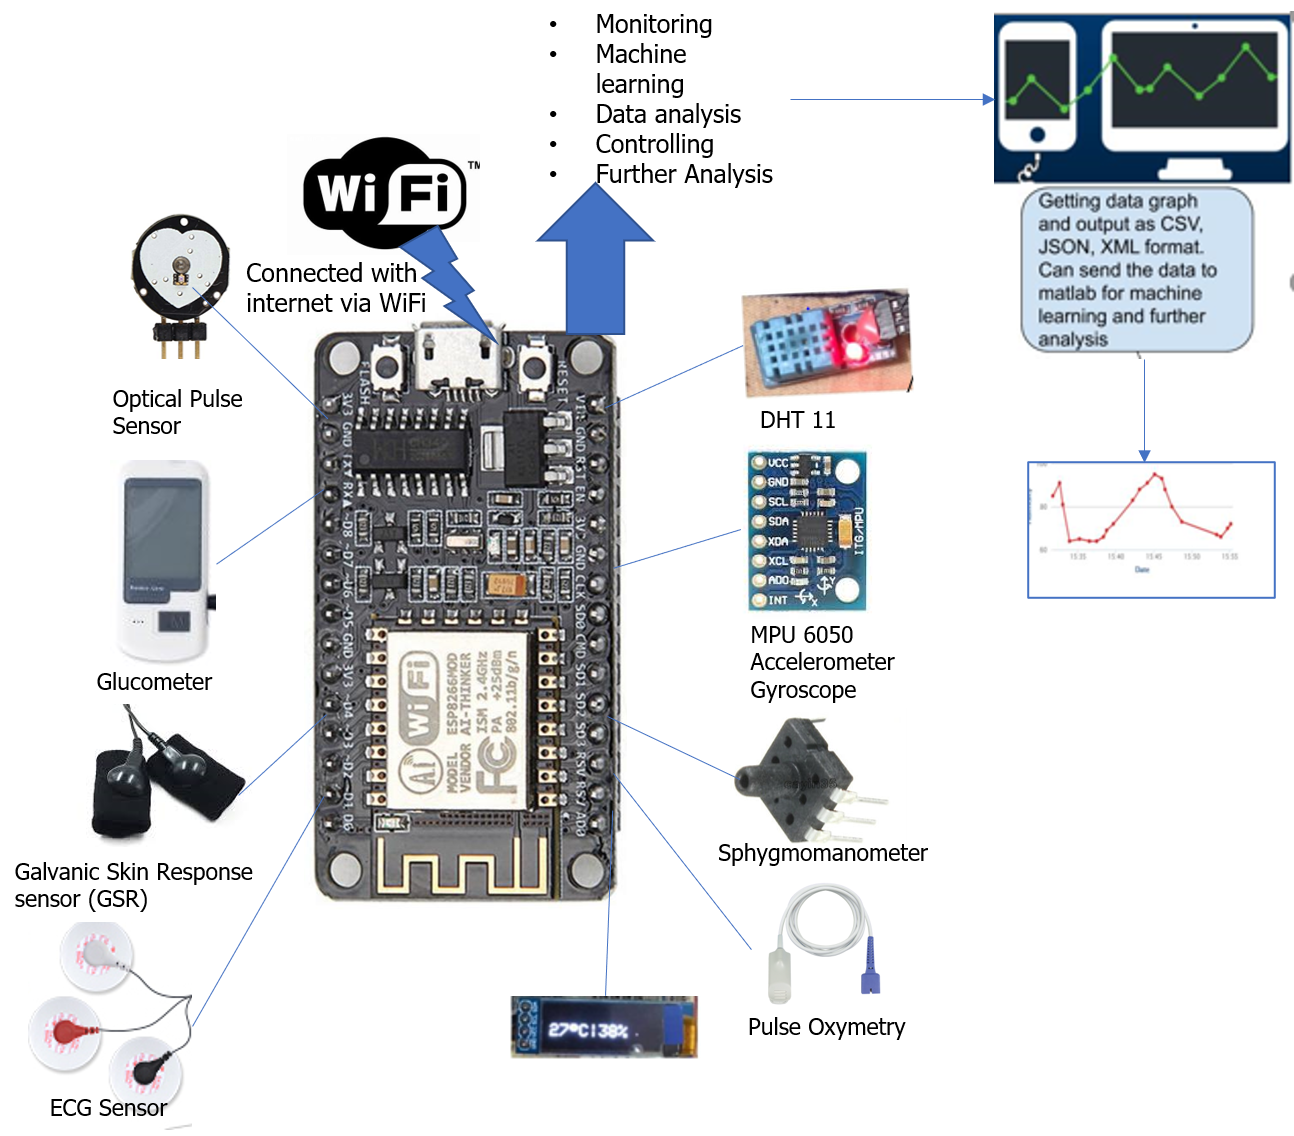
\includegraphics[width=5.5in]{Chap4/Circuit Diagram.png}
%     \caption{Circuit Diagram}
% \end{figure}